\chapter{Static dynamic bridge}
\label{chap:static_dynamic_bridge}

%\section{Coexistence between the static world and the dynamic world}
%introduction

In the programming world, there are three main families of programming language~\parencite{kwame.2017.qualitative}.
There are the \emph{compiled} programming, such as C, C++, Rust or Go. There are also the \emph{interpreted} programming
languages, such as Python, PHP, Lisp or Javascript. Finally, there are the hybrid programming languages, such as Java or
C\#, that have a fast compilation pass that compiles the source code into an intermediate bytecode. Then, this bytecode
is interpreted via an interpreter on the host (runner) machine.


\section{Introducing the static and dynamic bidge}

Many studies have carried out to compare the advantages and disadvantages of each family of programming
languages~\parencite{prechelt.2000.comparison,kwame.2017.qualitative,boehm.1984.economics}. In this thesis we focus
mainly on comparing the burden that are shouldered by the maintainers and the end-user.


\subsection{Languages types}

\paragraph{Compiled languages} From the maintainer point of view, there is a lot of burden to shoulder. First is the
binary generation which can be problematic in itself. Indeed, to generate a binary, there are many steps, as illustrated
in~\cref{fig:static.dynamic.compiled.compiletime}. First the compiler does a pass to generate machine code for each
translation unit. There can be as many machine code as there are architecture and/or operating system supported. The
maintainer may want to support different operating systems (last two windows and OSX version, a handful linux or unix
distributions, maybe mobile phone portages). Each of this OS requires its own bundle. Additionally, the hardware may
change, or the maintainer may want to take advantage of some specific hardware when available (like vectorized SIMD
instructions such as SSE4, XOP, FMA4, AVX-512, etc.): this also requires the maintainer to multiply the number of
binaries he compiles and distribute. Finally, the linker resolves the dependencies of the program and assemble the final
binary. At that time the maintainer has to sort out how he wants to bundle the dependencies of his program. Should he
statically link them alongside the binary and distribute them, at the risk of having the size of his binary exploding?
Or should he state that the user has to install the dependencies on his system (via a package manager for instance) so
that the binary can run? The burden of handling the dependencies is then shifted to the end-user when installing the
program.

\begin{figure}[htbp]
  \centering
  \includegraphics[width=.6\linewidth]{figs/static_compiletime}
  \caption{Compiled languages: compile-time}
  \label{fig:static.dynamic.compiled.compiletime}
\end{figure}


Usually the package manager, such as \emph{apt}, \emph{yum} or \emph{pacman}, solves this transparently for the end-user
and the programs works "out-of-the-box" once installed, as illustrated in~\cref{fig:static.dynamic.compiled.runtime}.
The downside is that the maintainer has to publish many bundles of his package where he wants it to be available.

\begin{figure}[htbp]
  \centering
  \includegraphics[width=.6\linewidth]{figs/static_runtime}
  \caption{Compiled languages: run-time}
  \label{fig:static.dynamic.compiled.runtime}
\end{figure}

\paragraph{Interpreted languages} From the maintainer point of view, this is the ideal standpoint. It is easier to
distribute software via an interpreted language because only the source code and, a dependency tree and the assets are
released in the bundle. All the burden about resolving the dependencies and installing the framework to run the script
is shouldered by the end-user that is using the program. Indeed, as shown in~\cref{fig:static.dynamic.dynamic.pipeline},
everything happens at runtime. The main advantage of this approach is to build a very rich ecosystem as distributing,
maintaining and using programs is very easy once integrated in a package manager (often delivered alongside the language
SDK natively, e.g. pip for python). However, the most notable disadvantage is the performance which is explained by the
fact that the source code is not compiled into optimized assembly code ready to be executed by the computer. Instead,
the interpreter must do all the work in one go and very often this is slow (at least the first pass). Nowadays,
interpreters differentiate two use cases. One is opening the console interpreter from the command line and typing
commands to get the immediate interpreted results. This use-case usually do not provide heavy optimization because it is
likely the user is prototyping his script and thus does not need it in the first place. The second use case is when the
interpreter parses files and/or libraries as a whole. In this use-case, it is likely that the file will not change, but
they will be used a lot. It is then relevant to pay a pass to generate intermediate bytecode that can be interpreted
faster for the future passes onward. As an example, the Python programming language has several implementations:
CPython, PyPy, Jython or IronPython. CPython generate intermediate bytecode in \texttt{*.pyc} files while Jython
IronPython and PyPy embed a Just-In-Time (JIT) compiler to generate resp. JVM bytecode, CLR (.NET) bytecode, a large
variety of bytecode format.

\begin{figure}[htbp]
  \centering
  \includegraphics[width=.6\linewidth]{figs/dynamic_pipeline}
  \caption{Interpreted languages: run-time}
  \label{fig:static.dynamic.dynamic.pipeline}
\end{figure}

\paragraph{Hybrid languages} The burden is shared evenly between the maintainer and the user, while remaining minimal.
Indeed, languages such as Java or C\# are in this category. Those programming languages need a compiling pass which is
designed to be fast, so that the feedback loop while prototyping remains fast. The result of the compilation is bytecode
which is then executed on an hosting Virtual Machine (VM) that the user must install on his computer. The main
advantages of this solution are the portability and the small distributed binary size. Indeed, in theory, any machine
supporting the VM may also support the program. Also, the as the VM execute the bytecode and resolve system
dependencies, the distributed binary does not need to embed any system dependency. Finally, the user has the advantage
of running a compiled program which provides fast user experience. The goal of hybrid languages is to ally advantages of
both compiled and interpreted languages; no dependency management for the user, one small binary to distribute for the
maintainer, good execution performance, and fast feedback loop when prototyping (fast incremental compilation), while
minimizing the downsides; usually a garbage collector is working inside the VM to handle memory allocations and
de-allocations. In this regard, both Java and C\# manage to achieve this feat quite elegantly. In theory, VM can further
increase performances by implementing hot code detection which would compile the bytecode into native optimized machine
code. This area is still a field of research to this day (c.f. Java
HotSpot~\parencite{xie.improving,kotzmann.2008.hotspot,halli.2016.java-hpc}).


\subsection{Static and dynamic informations}

Compiles programming languages usually have poor support of introspection facilities. At best, static reflection is
available at compile-time, but dynamic reflection is not an option. The structure of the program does not change at
runtime. Some flexibility exists when delving into the area of hot-swapping dynamic libraries at run-time, however this
techniques drags alongside security-related issues that injecting possible foreign machine code into one's program may
generate.
Interpreted programming languages usually have very developed introspection facilities. Dynamic reflection at
runtime is possible and some language, such as Common Lisp, even go further by allowing the developer to mutate the
program Abstract Syntax Tree (AST) at runtime (macro). This allows very powerful integrations such as defining one's own
DSL as if it was part of the core language itself.
Hybrid programming languages usually offers very good static and dynamic introspection facility at both compile-time and
runtime, even if it means that runtime facilities will hurt performances. Also, those languages are usually designed to
be able to hot-swap code at runtime. It is then possible to have the application running, recompile part of the binary
of the application, replace the old running binary by the new compiled one, all the while the application is running.

The next important step is to classify what information is known at \emph{compile-time} (machine/bytecode code
generation): we call it \emph{static} information; and what information is known at \emph{runtime} (program execution):
we call it \emph{dynamic} information. In image processing, have the following static informations:
\begin{itemize}
  \item Image's value type (unit8, rgb8, complex, etc.),
  \item Image's dimension size (1D, 2D, 3D, etc.),
  \item Architecture of the hardware hosting the program (x86, ARM, PowerPC, GPU, etc.).
\end{itemize}
On the other hand, we have the following dynamic informations:
\begin{itemize}
  \item Image's actual values,
  \item Image's actual size,
  \item Architecture of the hardware hosting the program (x86, ARM, PowerPC, GPU, etc.).
\end{itemize}

We notice that the architecture hosting the program is both an information which is static and dynamic. This translates
the complexity of this information. Indeed, the maintainer needs to guess the array of architectures he wants to support
and generate binaries for them (static). Also, the program needs to detect at runtime (dynamically) on which hardware he
is running to possibly take advantage of it to increase performances. This is an area of research on its own called
heterogeneous computing~\parencite{wong.2019.heterogeneous,brown.2019.heterogeneous}.


\subsection{Introducing our hybrid solution}

Image processing communities like to have bridges with interpretable language such as Python or Matlab, to interface
with their favorite tools, algorithms and/or facilities. As an example, with Python, the module
NumPy~\cite{oliphant.2006.numpy} is a community standard which is heavily used. Henceforth, to broaden the usage of our
library, we should be able to provide a way to communicate between our library and NumPy. There is always a need for
genecity in both C++ and Python. Indeed, in C++ genericity is achieved via template programming, which is static,
whereas in Python genericity is achieved via duck typing, which is dynamic, as shown
in~\cref{fig:static.vs.dynamic.genericity}.

\begin{figure}[htbp]
  \centering
  \subfloat[C++ static genericity]{
    \includegraphics[width=2in]{figs/cpp_static_code}
  }
  \hfil
  \subfloat[Python dynamic genericity]{
    \includegraphics[width=2in]{figs/python_dynamic_code}
  }
  \caption{C++ Static (a) vs. Python Dynamic (b) genericity.}
  \label{fig:static.vs.dynamic.genericity}
\end{figure}

On the one hand, static polymorphism induces no indirection in the generated code as the type is known at compile-time.
It is then possible to generate optimized code for specific types. It is not possible to add a new supported type at
runtime as the code has already been compiled. On the other hand, the dynamic polymorphism implies that there will be
indirections when executing the code. Indeed, the code first needs to dispatch onto the appropriate function handling
the input types to perform the operation properly. Nevertheless, it is possible to add new supported type at runtime
without recompiling the library binary.

From the maintainer point of view, however, only distributing the C++ templated source code is a showstopper to the
usability of his library by a Python user, because he does not hand over binaries. Indeed, one caveat of using C++
template programming is that the C++ compiler cannot generate a binary until it knows which type (of image, of value)
will be used. But the maintainer does not know this information and the user (on Python's end) does not want to
recompile the generic library code each time he has another set of types to exercise against. From here, there are still
multiple ways to achieve our goal.

The first option is to embed and distribute, alongside the library, a JIT compiler whose job would be to generate the
binaries and bindings just as they are used. This solution brings speed (excluding the first run that includes the
compilation time) and unrestrained genericity. However it bounds both user and maintainer to the specificities of a
compiler vendor and loose platform portability.

Another option is to type-erase (dynamic polymorphism) our types to enables the use of various concrete types through a
single generic interface. This would translate into a class hierarchy whose concrete classes are the leaves (thus, whose
value-types and dimensions are known). This induces a non-negligible performance overhead but enables us to keep the
genericity and portability at the cost of maintaining the class hierarchy.

Type generalization can also be considered. It is possible to cast everything into a super-type that is suitable for the
vast majority of cases. For instance, we could say that we have a super-type \texttt{image4D<double>} into which we can
easily cast sub-types such as \texttt{image2D<int>} or \texttt{image3D<float>}. Of course we would loose the generic
aspect and induce non negligible speed cost. Although portability is kept.

And finally there is the dynamic dispatch. It consists in embedding dynamic information at runtime about types, and
dispatch (think of switch/case) to the correct facility which can handle those types. The obvious caveat is the cost of
maintenance induced by the genericity as we would have a number of possible dispatches that grow in a multiplicative way
with the number of handled types. Which is not very generic. On the other hand there is almost no speed loss and the
portability is guaranteed. Theoretical models exist that could bring solutions to lower the number of dispatcher to
write, such as multi-method~\cite{pirkelbauer.2010.multimethods}. Unfortunately they are currently not part of C++.


\section{Designing the hybrid solution}

In Pylene we have chosen a hybrid solution between type-erasure and dynamic dispatch. The aim is to have a set of known
types for which we have no speed cost as well as continuing to handle other types to remain generic.
In~\cite{gossec.2019.pybind} we provide a facility to expose our generic code to Python. As seen in the previous
chapter, it is not possible to bind C++ source code to Python. We need to have a compiled binary implementing Python
binding (we chose Pybind11~\parencite{jakob.2017.pybind11}) in order to be able to call C++ code from Python. In order
to achieve the binding without sacrificing the genericity and the performances, we have designed a solution in two
steps. We do not want to provide an abstract interface that will resolve the calls to access data on the call-site via
virtual call because it would be very slow when the C++ code is executed. This would defeat the purpose of having to
rely on C++ in a first place. However, it is possible to convert an abstract class into an instantiated concrete generic
class whose template parameter are known. This requires, however, to enumerate all the possible cases. With modern C++,
it has become possible to design $n*n$ dispatch without gigantic switch-case clauses.


\subsection{First step: converting back and forth}

The first step of our solution consists in designing a buffer class that holds all the informations about an image:
dimension, underlying type, strides and pointer to data buffer. This class is named \texttt{ndimage\_buffer}. When
interfacing with Python, it is necessary to convert the Python image which is a \texttt{NumpPy.array} into our image
type and vise versa, converting our C++ image type back into a pythonimage. The purpose of this buffer image is to holds
all the information from the \texttt{NumpPy.array} to then instantiate a concrete C++ type. This process is illustrated
in~\cref{fig:type-erased.buffer}. The first pitfall here is due to a limitation from the abstraction interface used in
Python. Indeed, when using, for instance \emph{Scikit-Image}, it is not possible to differentiate a 2D multichannel
image from a 3D grayscale image. Indeed, the image is always broken down to its most simple value and a 2D multichannel
image is turned into a 3-dimensional \texttt{NumpPy.array} containing a single 8-bits channel, the last dimension
contains only 3 elements at max but can theoretically contain more. Indeed, there is no limitation embed in the used
abstraction which does not prevent that. To prevent this confusion, the C++ wrapper code may chose between two
strategies; first is to consider all 3D/1-channel image as 2D/RGB images by default, second is to let the user give the
information. For the sake of simplicity, we have chosen the first strategy.

\begin{figure}[htbp]
  \centering
  \includegraphics[width=.6\linewidth]{figs/type-erased_buffer}
  \caption{Bridge from Python to C++ via Pybind11 and a type-erased C++ class.}
  \label{fig:type-erased.buffer}
\end{figure}

From the point of view of a practitioner, the code on the call-site (python side) should be as follow:
\begin{minted}{python}
  from skimage import data
  import numpy as np
  import Pylena as pln # our python binding
  img = data.astronaut() # 2D-rgb8 image -> Numpy.array(ndim=3, dtype='uint8')
  # pln.<any_algorithm>(img)
\end{minted}

The C++ code contains lots of glue code necessary to expose the module to Python. In this thesis we have chosen to work
with Pybin11~\parencite{jakob.2017.pybind11} which provides a modern API and is actively being maintained and improved.
The glue code exposing the Python module from C++ is given in~\cref{appendix:static-dynamic-bridge.pylena}. In order to
have a seamless interaction between Python's \texttt{numpy.array} and C++, we need to define a proper strategy to
convert the Python type into the C++ type without copying all data around. Pybind offers us two possibilities to achieve
this. The first one is to use the buffer protocol to pass around numpy's buffer information to C++ in way so that C++
can properly bind the data into a proper C++ class. The second one is to use a custom type-caster to implicitly convert the python type
into a C++ type each time it is needed.

With the first method, one would need to write the following code on python's side:
\begin{minted}{python}
  np_img = data.astronaut() # 2D-rgb8 image -> Numpy.array(ndim=3, dtype='uint8')
  pln_img = pln.ndimage(np_img) # conversion into the C++ image type
  pln_img_ret = pln.<any_algorithm>(pln_img) # call to algorithm
  np_img_ret = pln_img.to_numpy(); # convert back into numpy.array
  # use np.<...>(np_img_ret) # use resulting image with numpy
\end{minted}
Whereas the second method would require the user to write the following code on python's side:
\begin{minted}{python}
  np_img = data.astronaut() # 2D-rgb8 image -> Numpy.array(ndim=3, dtype='uint8')
  np_img_ret = pln.<any_algorithm>(np_img) # implicit conversion with custom type-caster on C++ side
  # use np.<...>(np_img_ret) # use resulting image with numpy
\end{minted}
Removing this conversion step is the major reason we have chosen the second method: the custom type-caster. The C++ code
for this part is given in~\cref{appendix:static-dynamic-bridge.ndimage}.

We are now all set and are able to convert back-and-forth a python image into a C++ image and vice versa.

\subsection{Second step: multi-dispatcher (a.k.a. $\protect n*n$ dispatch)}

The second step of our hybrid solution is to dispatch the abstract buffer type coming from Python to an efficient
generic code. The naive way of doing so would be to include a gigantic switch-case clause in each algorithm
implementation and dispatch to the correct instantiated generic algorithm from there. Aside from being a nightmare to
maintain, the size of those clauses would grow several fold depending on the cardinality of the generic implementation.
For instance, for a generic dilation, there are 3 axis of cardinality: the underlying type, the dimension and the
structuring element shape. In the case where the library support 5 different structuring element shape, 10 underlying
types and 6 dimension for the image, the switch-case statement would need to dispatch over 300 clauses. Also, each
supported algorithm would need to have dispatcher. This solution defeat the purpose of genericity which is to write less
code in the first place. We needed to design a solution to implement those dispatchers while keeping our code short and
efficient. The idea we took to solve this problem comes from the design of a C++ feature, the variant, and especially
the visitor, applied to image processing, as in~\parencite{bourdev.2011.runtimedispatch} for instance. We need to have a
way to write the implementation of the algorithm once while enumerating all the possible cases. Also, if possible, the
list of supported types should be written once at one place for maintenance purpose.


\paragraph{Simple dispatcher}

We then had the idea of writing a dispatcher. This dispatcher lists all the supported types and call the given callbacks
forwarding the given arguments by instantiating a specific type. Let us try to expose to python, for instance, the
generic existing algorithm for thresholding a binary image. The Python call-site code will look like this:
\begin{minted}{python}
  img_grayscale = skimage.data.grass()
  pln.operators.binary_threshold(img_grayscale)
\end{minted}
On the C++ side, we want to avoid writing code that looks like this:
\begin{minted}{C++}
  mln::ndbuffer_image binary_threshold(mln::ndbuffer_image input) {
    auto dim = input.dim();
    auto tid = input.tid();
    switch(dim) {
      case 1: // 1D image
        switch(tid) {
          case UINT8:
            if(auto* image_ptr = input.template cast_to<uint8_t, 1>(); image_ptr)
              return mln::binary_threshold(*image_ptr);
          case RGB8:
            // error support only RGB8 images
        }
        break;
      case 2: // 2D image
        // ...
        break;
      // ... 3D, 4D, ...
    }
  }
\end{minted}
Instead, it is possible to separate the dispatching code and the logical code entirely by using a templated operator,
the same way we use lambdas in the pattern \texttt{std::variant}/\texttt{std::visit}. For our binary threshold example,
the operator be implemented just by writing the following code:
\begin{minted}{C++}
  // Operator templated by the dimension
  template <auto Dim>
  struct binary_threshold_op_t {
    // Function templated by the image type
    template <typename Img>
    mln::ndbuffer_image operator()(Img&& img) const {
      // Cast to a grayscale (information known) of the correct dimension
      if (auto* image_ptr = std::forward<Img>(img).template cast_to<std::uint8_t, Dim>(); image_ptr)
        // ACTUAL call to the generic algorithm
        return mln::binary_threshold(*image_ptr);
      else {
        std::runtime_error("Unable to convert the image to the required type.");
        return {};
      }
    }
  };
\end{minted}
This code allows us to dispatch over any number of dimensions. We are required to pass a grayscale image for the
algorithm so here the example is limited to dispatching over just one cardinality: the dimension. Let us now take a look
at how we can implement the dispatcher for our example to work. The dispatcher must take the dimension as first
parameter and any number of arguments to forward to the instantiated operator. The dispatcher then looks like the
following code:
\begin{minted}{C++}
template <template <auto> class Op, typename... Args>
auto dispatch_v(std::size_t dim, Args&&... args) {
  switch (dim) {
    case (1):
      return Op<1>{}(std::forward<Args>(args)...);
    case (2):
      return Op<2>{}(std::forward<Args>(args)...);
    case (3):
      return Op<3>{}(std::forward<Args>(args)...);
    /* ... */
  }
}
\end{minted}
The operator \texttt{Op} is instantiate with the correct dimension number and the the \texttt{operator()} (parenthesis)
is called while being forwarded the correct arguments. In our case, it will instantiate the type
\texttt{binary\_threshold\_op\_t<2>} and then call the function
\mintinline{c++}/binary_threshold_op_t<2>.operator()(input)/, forwarding the input image to the underlying algorithm.
Indeed, using the dispatcher is as simple as writing \mintinline{c++}/dispatch_v<binary_threshold_op_t>(input.dim(),
input);/

The main advantage of this approach is that we respect all the requirements. First the logical code is bounded in the
operator, second, the supported types are all listed in one place, once. Also, while our example is limited to one
cardinality, any number of dispatcher can be piped to one after another to achieve the cardinality wanted.


\paragraph{Double dispatcher}

Let us push our example to implement the mathematical morphology operator dilation. We now have two more generic axis to
cover: the structuring element shape and the underlying datatype. First, let us take a look at what the Python code may
look like:
\begin{minted}{python}
  img_grayscale = skimage.data.grass()
  rect = pln.se.rect2d(width=3, height=3)
  img_dil = pln.operators.dilate(img_grayscale, se)
\end{minted}
The first thing to notice is the need to add additional bindings to expose our C++ structuring elements. The glue code
to achieve this is given in~\cref{appendix:static-dynamic-bridge.se}. Let us take a look at our dilation operator:
\begin{minted}{C++}
template <auto Dim, typename T>
struct dilate_operator_t {
  template <typename Img, typename SE>
  mln::ndbuffer_image operator()(Img&& img, SE se) const {
    if (auto* image_ptr = std::forward<Img>(img).template cast_to<T, Dim>(); image_ptr)
      // ACTUAL call to the generic algorithm
      return mln::dilation(*image_ptr, se);
    else {
      std::runtime_error("Unable to convert the image to the required type.");
      return {};
    }
  }
};
\end{minted}
This operator needs double dispatch over two cardinalities: the dimension \texttt{Dim} and the value type \texttt{T}. We
can skip the dispatch of the structuring element's shape as we have made a \texttt{std::variant} of all the supported
structuring element supported for the sake of simplicity. Dispatching over the supported structuring elements can then
be offloaded upstream from the call to the double dispatch, just by calling \texttt{std::visit}. We can immediately
notice that there is an issue with our dilation operator. Indeed, there are two template parameters and our dispatcher
\texttt{dispatch\_v} does only handle one. We solve this issue by writing another intermediate operator dispatcher
\texttt{dilate\_operator\_intermediate\_t} serving as trampoline operator that will partially instantiate the final
operator \texttt{dilate\_operator\_t} along the dimension template parameter to feed it to the last dispatcher,
\texttt{dispatch\_t}:
\begin{minted}{C++}
template <auto Dim>
struct dilate_operator_intermediate_t {
  template <typename Img, typename SE>
  mln::ndbuffer_image operator()(Img&& img, SE&& se) const {
    // Partial instantiation
    return double_dispatch_t<dilate_operator_t, Dim>(
            input.sample_type(), std::forward<Img>(input), std::forward<SE>(se));
  }
};
\end{minted}
Dispatching the operator alongside two cardinalities (even three including the structuring element handled by
\texttt{std::variant}) would then become as simple as calling:
\begin{minted}{C++}
// dispatch the structuring elements through using std::visit for std::variant
return std::visit(
[&input](const auto& se_) { // dispatch over the trampoline
    return dispatch_v<dilate_operator_intermediate_t>(input.dim(), input, se_);
  }, se);
\end{minted}

In order for this to work, we need to piece together the final part of our puzzle, which is the double dispatch function
that will handle the last dispatch along the underlying data while forwarding the first dispatch along the dimension.
This dispatcher works the same as the simple one (\texttt{dispatch\_v}) but take an additional template parameter (here
\texttt{Dim}) that will be forwarded as-is to the given operator \texttt{Op}. The implementation then looks like this:
\begin{minted}{C++}
template <template <auto, typename> class Op, auto Dim, typename... Args>
auto double_dispatch_t(type_id tid, Args&&... args) {
  switch (tid) {
    case (type_id::INT8):
      return Op<Dim, std::int8_t>{}(std::forward<Args>(args)...);
    case (type_id::UINT8):
      return Op<Dim, std::uint8_t>{}(std::forward<Args>(args)...);
    case (type_id::DOUBLE):
      return Op<Dim, double>{}(std::forward<Args>(args)...);
      /* ... */
  }
}
\end{minted}
We have now presented all the techniques and design required to build operators that are agnostic from the supported
data-types, dimensions and/or additional data such as structuring elements. Indeed, the maintainer has gathered all the
logic about listing the supported data types and dimension in one place: the custom dispatcher. He just needs to
maintain those to enable full support for all exposed algorithm, by default. This hybrid solution mixes type-erasure and
modern C++ facilities to allow maximum performance. Indeed, the dispatch is done before entering algorithms and the
custom type-caster facility allows us to plug directly into the Python image without having any unnecessary copies. The
only caveat would be the code bloat incurred by all the explicit instanciation leading to compiling a larger and larger
binary the more algorithms are being exposed. This can lead to performances issues due to pre-fetching memory
optimization missed and code locality issues~\parencite{badawy.2001.locality}. Another point not covered right now would
be a way to support arbitrary data types, possibly injected from Python, into C++. Indeed, our hybrid solution only
support the types provided by the library and listed in the dispatchers. It will instantiate all the code relative to
them and support all of the combinations but the user may be tempted to plug a user-defined type from Python as an
underlying image data-type. To allow this use-case, we introduce a new concept: the \emph{value-set}. The value-set is a
standard way manipulate the underlying values. Through type-erasure, we can either manipulate known underlying value
type with native facilities (near-zero overhead), or fallback to a virtual call that may report an error, or callback
user-provided Python routine to manipulate unknown user values.


\subsection{Third and final step: type-erasure \& the value-set}

As common thread in this section, we will work on the morphological \emph{stretch} algorithm which is naively defined as
followed:
\begin{minted}{C++}
template <class T>
mln::image2d<float> naive_stretch(const mln::image2d<T>& src)
{
  mln::image2d<float> res  = mln::transform(src, [](auto val) -> float {
    auto max = std::numeric_limits<T>::max();
    return static_cast<float>(val) / static_cast<float>(max);
  });
  return res;
}
\end{minted}

\begin{figure}[htbp]
  \centering
  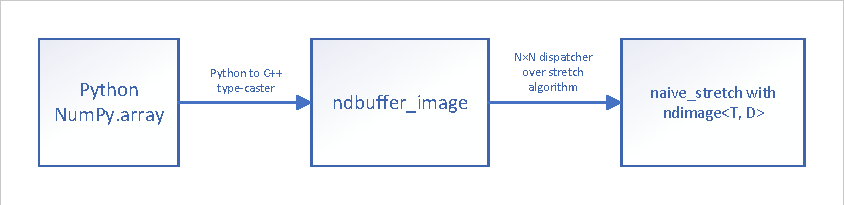
\includegraphics[width=.8\linewidth]{figs/static_dynamic_bridge/nxndispatch_pipeline}
  \caption{Python to C++ pipeline algorithm through the $n*n$ dispatcher.}
  \label{fig:static_dyn.nxndispatcher}
\end{figure}

We can represent the pipeline calling this algorithm from Python in~\cref{fig:static_dyn.nxndispatcher}.

\paragraph{Introducing the value-set}

The \emph{value-set} is an abstraction layer around common operations needed when implementing an image processing
algorithm such as an addition, a multiplication, a type conversion, getting the maximum etc. It can be defined in C++ as
a class template whose parameter is the manipulated type. The following code shows how to define a value-set:
\begin{minted}{C++}
template <class T = void>
struct value_set {
  template <class U>
  U cast(T v) const { return static_cast<U>(v); }

  T max() const noexcept { return std::numeric_limits<T>::max(); }
  T min() const noexcept { return std::numeric_limits<T>::min(); }
  /* inf, sup, ... */

  T add(T l, T r) const noexcept { return l + r; }
  T sub(T l, T r) const noexcept { return l - r; }
  /* mod, pow, min, max, ... */
};
\end{minted}
We can see that the default parameter of the class template is \texttt{void}. Indeed, we are inspired by what was
implemented in the standard library for \texttt{std:less} and providing a default (void) specialization in order to
improve the usability. The following code shows how to implement this specialization:
\begin{minted}{C++}
template <>
struct value_set<void> {
  template <class U, class T>
  U cast(T&& t) const { return static_cast<U>(std::forward<T>); }

  template <class T, class U>
  auto add(T&& l, U&& r) const noexcept { return std::forward<T>(l) + std::forward<U>(r); }
  template <class T, class U>
  auto sub(T&& l, U&& r) const noexcept { return std::forward<T>(l) - std::forward<U>(r); }
  /* ... */
};
\end{minted}
The full code of the value-set is given in~\cref{appendix:static-dynamic-bridge.mm.vs}. The template parameter is
shifted from the class to the member functions. It is also important to note that the member function are not static,
which requires to instantiate the \texttt{value-set} before using it. It may sound like a disadvantage at first glance
but it can be turned into an advantage later on. Indeed, this design allows a subclass to hold member variables which
will be crucial for injecting user-types from python.

Now that we have designed how our value-set is intended to work, we can deduce that an image is able to provide its own
value-set. Indeed, an image knows what values it holds and thus is able to instantiate the proper value-set
corresponding to this type. The member function returning the value-set in the class template \texttt{ndimage<T, D>} is
then implemented as follow:
\begin{minted}{C++}
template <class T, std::size_t D>
class ndimage {
  /* ... */
  auto get_value_set() const noexcept {
    return value_set<T>{};
  }
};
\end{minted}

\begin{figure}[htbp]
  \centering
  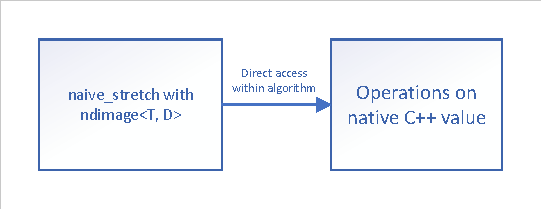
\includegraphics[width=.8\linewidth]{figs/static_dynamic_bridge/naive_stretch}
  \caption{Naive stretch algorithm, pipeline to perform operations on values.}
  \label{fig:static_dyn.naive_stretch}
\end{figure}

Let us recall our naive stretch algorithm presented earlier. The pipeline representing the operations on values inside
the algorithm is presented in~\cref{fig:static_dyn.naive_stretch}. Typically, this algorithm performs three operations
that are the responsibility of a value-set: getting the max, performing a cast, and performing a division. The first
step is then to use the value set shown above to abstract away those operations. The algorithm then becomes:
\begin{minted}[linenos,highlightlines={4-5,7,8-9,10}]{C++}
template <class T>
mln::image2d<float> fast_stretch(const mln::image2d<T>& src)
{
  auto                vs   = src.get_value_set();     // value-set for T
  auto                vs_f = mln::value_set<float>{}; // fast value-set for float
  mln::image2d<float> res  = mln::transform(src, [&vs, &vs_f](auto val) -> float {
    auto max  = vs.max();                     // returns T
    auto fval = vs.template cast<float>(val); // returns float
    auto fmax = vs.template cast<float>(max); // returns float
    return vs_f.div(fval, fmax);              // div directly returns float
  });
  return res;
}
\end{minted}

\begin{figure}[htbp]
  \centering
  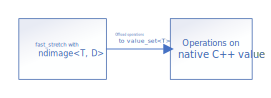
\includegraphics[width=.8\linewidth]{figs/static_dynamic_bridge/fast_stretch}
  \caption{Fast stretch algorithm, pipeline to perform operations on values.}
  \label{fig:static_dyn.fast_stretch}
\end{figure}

We instantiates the value-set we will need (for \texttt{T} values and \texttt{float} values) on lines 4 and 5. Then the
maximum value is obtained via the value-set of \texttt{T} on line 7. Then a cast is performed via the value-set to get
floating point value on lines 8 and 9. Finally a floating point division is performed on line 10 via the formerly
instantiates floating point value-set defined on line 5. Indeed, using the value-set instantiated for \texttt{T} would
have performed an Euclidean division and which would have resulted in a bug. Calling this algorithm from python is as
simple as \mintinline{python}/ret = pln.fast_stretch(input)/ once exposed. The pipeline representing the actual
operations in the algorithm to access values is shown in~\cref{fig:static_dyn.fast_stretch}. The glue code to expose
this algorithm is givenin~\cref{appendix:static-dynamic-bridge.mm.algos}.

\paragraph{Type-erasure interface for value-set}

Moving one step further, we ultimately want to be able to dynamically inject a value-set into our algorithm. In order to
achieve this feat, we need to design an abstract value-set as an interface so that a user can sub-class it and provide
his own value set. This abstract value-set needs to work with \texttt{std::any} as input value-type in order to provide
a generic interface. Here, the genericity is achieved via type-erasure (the input value is type-erased into a
\texttt{std::any}). The interface would look like (full code is given in~\cref{appendix:static-dynamic-bridge.mm.vs}):
\begin{minted}{C++}
struct abstract_value_set {
  virtual ~abstract_value_set() {}

  virtual std::any max() const = 0;
  /* min, sup, inf, ... */

  virtual std::any add(const std::any& l, const std::any& r) const  = 0;
  virtual std::any div(const std::any& l, const std::any& r) const  = 0;
  /* sub, mult, ... */
};
\end{minted}
The important part here is to notice that all values (returned and passed as argument) are now type-erased behind a
\texttt{std::any}. From this interface, it is trivial to define the canonical sub-classes for trivial types. We do this
by defining the class template \texttt{concrete\_value\_set} which is able to generate a concrete interface for every
given template type. The implementation will look like this:
\begin{minted}{C++}
template <typename T>
struct concrete_value_set : abstract_value_set {
  ~concrete_value_set() override {}

  template <class U>
  std::any cast(std::any v) const { return {static_cast<U>(std::any_cast<T>(v))}; }

  std::any max() const override { return {std::numeric_limits<T>::max()}; };
  /* min, sup, inf, ... */

  std::any add(const std::any& l, const std::any& r) const override {
    return {std::any_cast<T>(l) + std::any_cast<T>(r)};
  }
  std::any div(const std::any& l, const std::any& r) const override {
    return {std::any_cast<T>(l) / std::any_cast<T>(r)};
  }
  /* sub, mult, ... */
};
\end{minted}
This concrete value-set implement simple dispatch via casting the type-erased \texttt{std::any} into the wanted value
type to properly perform the operation. Thanks to this implementation, we are able to rewrite our stretch algorithm
using this value-set to perform its operations. The new algorithm now looks like this:
\begin{minted}[linenos,highlightlines={4-5,7,8-9,10}]{C++}
template <class T>
mln::image2d<float> virtual_dispatch_stretch(const mln::image2d<T>& src)
{
  auto                vs   = mln::concrete_value_set<T>{};     // value-set for T
  auto                vs_f = mln::concrete_value_set<float>{}; // value-set for float
  mln::image2d<float> res  = mln::transform(src, [&vs, &vs_f](auto val) -> float {
    auto anymax  = vs.max();                                 // returns std::any
    auto fanyval = vs.template cast<float>(val);             // cast to float in std::any
    auto fanymax = vs.template cast<float>(anymax);          // cast to float in std::any
    return std::any_cast<float>(vs_f.div(fanyval, fanymax)); // div returns float
  });
  return res;
}
\end{minted}

\begin{figure}[htbp]
  \centering
  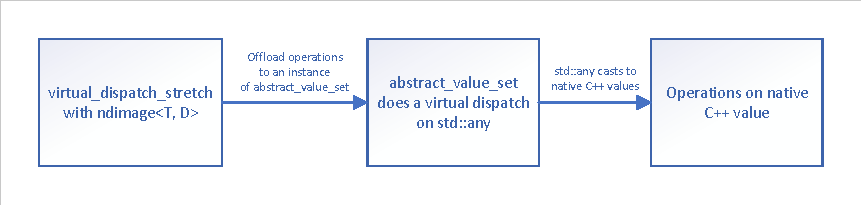
\includegraphics[width=.8\linewidth]{figs/static_dynamic_bridge/virtual_dispatch_stretch}
  \caption{Virtual dispatch stretch algorithm, pipeline to perform operations on values.}
  \label{fig:static_dyn.virtual_dispatch_stretch}
\end{figure}

This algorithm uses two value sets (l.4 and l.5), one to get the maximum value with regard of the original underlying
value type in the image \texttt{T} (l.7) and to properly cast the values into float values (l.8-9). The other one is
used to perform the floating point division (l.10). This algorithm is almost identical to the one given for
\texttt{fast\_stretch} earlier. Only the lines instantiating the value-set changes (l. 4-5) as well as the line handing
over the result (l. 10) where we added a downcast from \texttt{std::any}. The pipeline presenting the operations needed
to access values is presented in~\cref{fig:static_dyn.virtual_dispatch_stretch}.


\paragraph{Going forward: type-erasing the value entirely}

The need may arise where the user wants to handle images where the input value is abstracted away behind a type-erased
type. This value-type would then embed its own value set able to perform operations (as a pointer for instance). This
fallback would allow writing such code possible:
\begin{minted}[highlightlines={10}]{C++}
class type_erased_value {
  type_erased_value add(const type_erased_value& rhs);
  /* ... */
};

void my_algo(ndimage<type_erased_value, Dim> img1,
              ndimage<type_erased_value, Dim> img2) {
  ndimage<type_erased_value, Dim> img_out = /* ... */;
  for (auto [v1, v2, out] : zip(img1.values(), img2.values(), img_out.values())) {
    out = v1.add(v2); // the value knows how to perform the addition
  }
}
\end{minted}

This code enables fallback when all the supported values have been exhausted. For instance, when considering the
previously defined \texttt{abstract\_value\_set}, when attempting to dispatch over all the supporting native C++ type
unwrapped from the given \texttt{std::any}, if no type is matched, we can attempt one final unwrap to this type-erased
value which is aware itself of how to perform the operation. In pseudo-code it breaks down to the following logic:
\begin{minted}[linenos,highlightlines={3,4-5,6,9-10}]{C++}
std::any value_set<type_erased_value>::add(const std::any& lhs, const std::any& rhs){
  abstract_value_set* vs = lhs.get_embedded_vs();
  if (lhs.type() == typeid(int) && rhs.type() == typeid(int)) {
    auto ret = std::any_cast<int>(lhs) + std::any_cast<int>; // unwrap, do the work
    return std::any{ret}; // rewrap with the vs
  } else if (lhs.type() == typeid(float) && rhs.type() == typeid(float)) {
    /* ... same ... */
  } else {
    auto te_lhs = std::any_cast<type_erased_value>(lhs); // last attempt
    return lhs.add(rhs); // fallback on embedded value-set
  }
}
\end{minted}
First step is to conditionally attempt to cast the type-erased value over the supported native values (lines 3 and 6).
When the type is supported then we unwrap it and perform the operation before rewrapping it in a \texttt{std::any} and
returning it. If we could not unwrap the value into a supported value-type, we make a last attempt on line 9 into our
type-erased value-type. If this attempt succeeds, we rely on the fact that this value-type is aware of its own value-set
and embed it to perform the required operation on line 10. The full code of the implementation for this value-set aware value-type is given
in~\cref{appendix:static-dynamic-bridge.mm.vs}. We have relied on metaprogramming techniques in order to efficiently
write the code that will do the work.

Thanks to this technique, we are able to write another version of our stretch algorithm, as followed:
\begin{minted}[linenos,highlightlines={8-12,13-14,17-18,20,22,23}]{C++}
template <class T>
mln::image2d<float> stretch_virtual_dispatch_type_erased_value(const mln::image2d<T>& src)
{
  auto                vs   = mln::concrete_value_set<T>{};     // value-set for T
  auto                vs_f = mln::concrete_value_set<float>{}; // value-set for float
  mln::image2d<float> res  = mln::transform(src, [&vs, &vs_f](auto val) -> float {
    // simulate having an image<type_erased_value>
    auto anyval = std::any{val}; // std::any of T
                                  // type_erased_value of std::any of T aware of value-set of T
    auto abs_anyval = mln::type_erased_value{anyval, vs};
    // instantiate a value-set for type_erased_value
    auto abs_vs = mln::value_set<mln::type_erased_value>{abs_anyval};
    auto anyabs_anymax =
        abs_vs.max(); // returns std::any of type_erased_value
                      // cast underlying std::any of type_erased_value of std::any of T into
                      // std::any of type_erased_value of std::any of float aware of value-set for float
    auto anyabs_fanyval = abs_vs.template cast<T, float>(std::any{abs_anyval}, &vs_f);
    auto anyabs_fanymax = abs_vs.template cast<T, float>(anyabs_anymax, &vs_f);
    // dispatch on known type, find a type_erased_value, then call
    // anyabs_fanyval.div(anyabs_fanymax) to perform division which will call
    // the underlying value-set for float for this operation
    auto anyabs_fanyret = abs_vs.div(anyabs_fanyval, anyabs_fanymax);
    // convert result back into float for returning to the image
    auto anyfret = std::any_cast<mln::type_erased_value>(anyabs_fanyret).val();
    return std::any_cast<float>(anyfret);
  });
  return res;
}
\end{minted}

\begin{figure}[htbp]
  \centering
  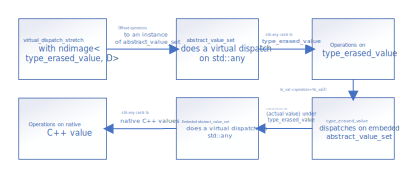
\includegraphics[width=.8\linewidth]{figs/static_dynamic_bridge/virtual_dispatch_type_erased_value_stretch}
  \caption{Virtual dispatch stretch algorithm with a type-erased value, pipeline to perform operations on values.}
  \label{fig:static_dyn.virtual_dispatch_type_erased_value_stretch}
\end{figure}

This version is verbose because we do not yet support mln::image2d<type_value_value> as a proper image type. Thus we
need to first convert the value of type \texttt{T} into the value-set aware type-erased value type. This work is done on
lines 8 to 12. Then on lines 13 to 20 we perform the actual work on the values. This is where the dispatch mechanic,
whose pipeline is shown in detail in~\cref{fig:static_dyn.virtual_dispatch_type_erased_value_stretch}, will happen.
Finally, on lines 22 and 23, we unwrap the previously wrapped type-erased value into a float to return for the
algorithm.


\paragraph{Everything comes to a full circle: injecting a value-set from Python}

We have seen how to write an algorithm independently from ths its underlying types on C++ side thanks to relying on an
abstraction layer: the value-set. This enables one fundamental feature which is code injection from Python. Indeed, if
we suppose every python value is a \texttt{pybind11::object}, which is the generic way to refer to a
non-trivially-convertible Python type we can write a value-set handling this value type. The value-set handling python
data-type would then provide the following interface:

\begin{minted}[linenos,highlightlines={4,8,10,15-17,21-23,27}]{C++}
template <>
struct value_set<pybind11::object> : abstract_value_set
{
  value_set(pybind11::object python_vs_instance): vs_instance_(python_vs_instance) {}
  ~value_set() override {}

  template <typename U>
  std::any cast(const std::any& v) const { /* ... */ }

  std::any max() const override { {vs_instance_.attr("max")()}; }
  /* min, sup, inf, ... */

  std::any add(const std::any& l, const std::any& r) const override
  {
    auto pyl = std::any_cast<pybind11::object>(l);
    auto pyr = std::any_cast<pybind11::object>(r);
    return {vs_instance_.attr("add")(pyl, pyr)};
  }
  std::any div(const std::any& l, const std::any& r) const override
  {
    auto pyl = std::any_cast<pybind11::object>(l);
    auto pyr = std::any_cast<pybind11::object>(r);
    return {vs_instance_.attr("div")(pyl, pyr)};
  }
  /* max, min, sub, mult, ... */
private:
  pybind11::object vs_instance_;
};
\end{minted}

In this code we can clearly see at lines 4 and 27 that we are storing our Python's value-set instance into our class.
This is possible due to the fact that our value-set abstraction is not providing static class function but member
function. Hence, it is possible to offload the work of the value-set to a member variable at lines 10, 15-17 and 21-23
that will call the Python's value-set and get the wanted result. Also, at line 8 we use multiples techniques at once to
get the correct resulting cast from a Python type. Indeed, the cast is done on Python side before being casted back into
the corresponding C++ type. As such, we have to translate the wanted C++ type information into Python type information
to request the cast. Once the cast is done, we need to unwrap the python type into the corresponding C++ type and rewrap
it into our, now favorite, \textt{std::any}. The full implementation of this facility is given
in~\cref{appendix:static-dynamic-bridge.mm.vs.py_value_set.hpp}.

On this particular matter, the user will find a Python abstract class to implement in order for his value-set to be
usable by the library. This abstract class is defined by the following Python code:

\begin{minted}{python}
from abc import ABC, abstractmethod
from typing import Any
import math, importlib

class AbstractValueSet(ABC):

  @abstractmethod
  def cast(self, value: Any, type_): pass
    if type_ in ["int", "float", "bool", "str"]:
      module = importlib.import_module('builtins')
      cls = getattr(module, type_)
      return cls(value)
    else:
      raise ValueError()

  @abstractmethod
  def max(self): return math.inf

  @abstractmethod
  def min(self): return -math.inf

  # ...

  @abstractmethod
  def add(self, lhs: Any, rhs: Any) -> Any: return lhs + rhs

  @abstractmethod
  def sub(self, lhs: Any, rhs: Any) -> Any: return lhs - rhs

  # ...
\end{minted}

This abstract class provide a facility to cast a value into a given type from its representation as a string. It also
provides default / standard way of computing values. Those methods needs to be overridden by a child class as they are
all tagged with the \texttt{@abstractmethod} attribute.

\FIXME{TODO, finish this part.}

Now, let us make our own custom Python data structure containing a value. Let us name our class \texttt{MyStruct} as in
the following code:

\begin{minted}{Python}
from typing import Any
class MyStruct:
  v_: Any
  def __init__(self, v: Any): self.v_ = v
  def getV(self) -> Any:      return self.v_
  def setV(self, v: Any):     self.v_ = v
\end{minted}

Now we want to use this custom structure in an image we pass to the C++ library. The following Python code will not
work:

\begin{minted}{Python}
img = np.array(
  [MyStruct(1), MyStruct(2), MyStruct(6.5), MyStruct(3.14)],
  ndmin=1)
pln_img = pln.ndimage(img, is_multichannel=false)
\end{minted}

Indeed, the image's value-type is a \texttt{pybind11::object} which requires the C++ code to fallback on the
corresponding value-set specialization. However, in order to construct a value-set of that specialization, we are
missing a parameter: the \texttt{pybind11::object} value-set offloading the work to Python. The next step is then to
declare our custom value-set on Python side shown on the following code:

\begin{minted}{Python}
from typing import Any

class MyValueSet(AbstractValueSet):
  def get_MyStruct_val__(self, v: Any):
    return v.getV() if isinstance(v, MyStruct) else v

  def cast(self, value: Any, type_):
    return super().cast(self.get_MyStruct__(value), type_)

  def max(self): return super().max()

  def min(self): return super().min()

  def add(self, lhs: Any, rhs: Any) -> Any:
    return MyStruct(super().add(self.get_MyStruct__(lhs), self.get_MyStruct__(rhs)))

  def sub(self, lhs: Any, rhs: Any) -> Any:
    return MyStruct(super().sub(self.get_MyStruct__(lhs), self.get_MyStruct__(rhs)))
\end{minted}

Now it is possible to write the following code:
\begin{minted}{Python}
  img = np.array(
    [MyStruct(1), MyStruct(2), MyStruct(6.5), MyStruct(3.14)],
    ndmin=1)
  pln_img = pln.ndimage(img, is_multichannel=false, value_set=MyValueSet())
\end{minted}

And on the C++ side there are just small trivial adaptations to do to forward the \texttt{pybind11::object} to the
\texttt{ndimage\_from\_buffer} function so that it is then correctly forwarded into the resulting
\texttt{mln::ndbuffer\_image}, thus accessible from any algorithms. There is another way of achieving the exact same
result which consist of having a concrete value-set Python class inheriting an abstract value-set C++ class. This is
rendered possible by using a trampoline on the C++ side to define a special C++ class (with macros provided by pybind).
Afterwards, it is possible to define a Python class in Python code inheriting from the trampoline intermediate C++
class. Then the user implement the pure virtual member function with Python code. Thanks to polymorphism, it is then
possible to pass this child class back to a C++ function as if it was the C++ parent class. Whichever solution is
selected, the performances remain equally bad as Python code do the work in both case.

Indeed, while it works and enables the user to construct \texttt{numpy.array} of custom Python type and pass them to the
library with the corresponding value-set for it to "just work", the performance is greatly impacted. As a matter of
fact, the computation is no longer done on the C++ side with optimized, vectorized instructions. Instead, a callback to
Python is done in order to get the result. It is important that the user keep in mind that custom python types are be
supported by the library by providing a value-set at the cost that the resulting performances will literally be blown
away. This may be sufficient for prototyping and tinkering however the user must consider implementing his own type on
the C++ side when time comes to write production code.

\section{Performances \& overhead}

% Native value-set with native C++ value-type: 0.0093sec
% Value-set with virtual dispatch with native C++ value-type: 0.1213sec
% Value-set with virtual dispatch with C++ type-erased values: 1.0738sec
% Injected Python value-set with native C++ value-type: 21.5444sec

\begin{table}[htbp]
  \begin{tabular}{l|ccc}
    \toprule
    Dispatch type                                               & Compute Time & $\Delta{}$Compute Time \\ \midrule
    Native value-set with native C++ value-type                 & $0.0093s$    & $0$                    \\
    Value-set with virtual dispatch with native C++ value-type  & $0.1213s$    & $\times 13$            \\
    Value-set with virtual dispatch with C++ type-erased values & $1.0738s$    & $\times 115$           \\
    Injected Python value-set with native C++ value-type        & $21.5444s$   & $\times 2316$          \\
    \bottomrule
  \end{tabular}
  \caption{Benchmarks of the pipeline \cref{fig.view.comp.sub_bg} on a dataset (12 images) of 10MPix images. Average
    computation time and memory usage of implementations with/without \emph{views} and with OpenCV as a baseline.}
  \label{table:static.dynamic.perfs}
  %\vspace{-1em}
\end{table}

\section{JIT-based solutions: pros. and cons.}

Our hybrid solution certainly has advantages but the huge disadvantage is the slowness of injecting our own types from
the Python side. There exists another solution that this thesis did not have the opportunity to study in-depth. This
solution is based on a known technology: the Just-In-Time (JIT) compilation which has been previously illustrated
in~\cref{fig:static.dynamic.dynamic.pipeline}. Indeed, it is a technology already used by interpreted languages such as
Java or PHP to generate on-the-fly native and optimized machine code for the section of the source code that is
considered "hot" by the interpreter. A source code is "hot" when it is executed a lot: the end-user would gain paying
the compilation time once to have this code executed faster several times later on. When applying this strategy to our
problematic, it would mean that the user must be able to compile native machine code from the templated generic C++ code
by injected the requested type when it is used. Such an operation shift heavily the burden on the user and it is
well-known that compiling C++ code is notably \emph{complicated} and \emph{slow}. In addition, the library needs to be
able to auto-generate python-binding once the code is compiled. There are several solutions to achieve this process.

The first solution is to basically use system call to the compilers to actually \emph{compile} C++ code once the
templated types are known and explicitly instanciated in the source code. This solution requires careful code-generation
design and that the user actually possess a compiler on his computer. Furtheremore, the user must resolve all the
library dependencies, such as \emph{freeimage} for IO etc. This solution was engineered in the
library~\parencite{demaille.2013.vcsn}. Indeed, each time the user declared a new automata in his jupyter notebook,
corresponding source code is compiled in the foreground and then cached. It is a very perilous solution to implement
when the final execution environment (OS, installed software) is not well-known in advance. Nowadays, the issue may be
lesser, however, it still requires to maintain both the library and the container solution to use it.

The second solution is to use Cython~\parencite{behnel.2010.cython}. It is a transpiling infrastructure which transform
a Python source code directly into C-language source code so that it can be compiled by a standard C compiler just by
linking against the Python/C API. This remove the burden of writting the careful code-generation routine, system-calls
to the C++ compiler and removes the need to resolve all the dependencies. This infrastructure takes care of everything
for the user. Also, by transpiling it into C code, it is faster because a C compiler is faster than a C++ compiler.
Cython even support C++ template code~\parencite{behnel.2022.cython-template} which is mandatory for our use-case.

The third solution consists in relying on recent projects that are all relying on the LLVM infrastructure. We can
notably note Autowig~\parencite{fernique.2018.autowig}, Cppyy~\parencite{wimtlplavrijsen.2016.cppyy} and
Xeus-cling~\parencite{quantstack.2021.xeus-cling}. Autowig has in-house code based on LLVM/Clang to parse C++ code in
order to generate and compile a Swig Python binding using the Mako templating engine. Autowig, coupled with Cython would
permit the user to, for instance, generate C code related to a custom Python structure. Then a simple call to Autowig
will parse the C code and inject it into the C++ library to generate the appropriate bindings for the user. As for
Cppyy, it is based on LLVM/Cling, a C++ interpreter, and can directly interpret C++ code from a python string. This
allow for easy injection of custom types, be they in Python code (transpiled with Cython) or C++ code (directly
interpreted by Cling). Afterwards, the infrastructure generates the appropriate binding from the templated C++ library
for the injected type. Finally, Xeus-cling is a ready-to-use jupyter kernel and allow the usage of C++ code directly
from within a notebook. This completely bypass the need of a Python binding in the first place and allow the user to use
the library from within the notebook as if he was using a Python library. However all those infrastructure come with a
hefty cost in term of binary size. Indeed, a C++ compiler is not small and embarking it alongside the image processing
library can easily impact greatly the final binary. Without the LLVM infrastructure the binary may weight around 3MB.
With the LLVM infrastructure, the binary weight at the bare minimum 50MB. Also, these solutions may not be immediately
faster. Indeed, when prototyping back and forth with a variety of types, the user may not be eager to wait for long
compilations times each time he is testing with a an iteration of his work. Despite those facts, those solutions offers
great avenue of research for the future and the author is eager to thread those paths.
